\documentclass[11pt,a4paper]{article}

% ---------- packages ----------
\usepackage[margin=2.3cm]{geometry}
\usepackage{amsmath,amssymb}
\usepackage{graphicx}
\usepackage{xcolor}
\usepackage{listings}
\usepackage{hyperref}
\usepackage{enumitem}
\usepackage{booktabs}
\usepackage{titlesec}
\usepackage{fancyhdr}
\usepackage{tikz}
\usetikzlibrary{trees,positioning}

% ---------- hyperref colours ----------
\hypersetup{
    colorlinks=true,
    linkcolor=black,
    urlcolor=blue!60!black,
    citecolor=blue!60!black
}

% ---------- listings style for C++ ----------
\definecolor{codebg}{RGB}{248,248,248}
\definecolor{codekw}{RGB}{0,0,160}
\definecolor{codecm}{RGB}{40,120,40}
\definecolor{codestr}{RGB}{160,0,40}

\lstdefinestyle{cpp}{
    language=C++,
    backgroundcolor=\color{codebg},
    basicstyle=\ttfamily\footnotesize,
    keywordstyle=\color{codekw}\bfseries,
    commentstyle=\color{codecm}\itshape,
    stringstyle=\color{codestr},
    numbers=left,
    numberstyle=\tiny\color{gray},
    stepnumber=1,
    breaklines=true,
    frame=single,
    framesep=4pt,
    showstringspaces=false,
    tabsize=2,
    captionpos=b
}
\lstdefinestyle{plain}{
    backgroundcolor=\color{codebg},
    basicstyle=\ttfamily\footnotesize,
    breaklines=true,
    frame=single,
    framesep=4pt,
    tabsize=2
}

% ---------- header ----------
\pagestyle{fancy}
\fancyhf{}
\fancyhead[L]{2-3-4 Tree Assignment}
\fancyhead[R]{\thepage}

\titleformat{\section}{\large\bfseries\color{blue!40!black}}{\thesection.}{0.6em}{}
\titleformat{\subsection}{\normalsize\bfseries}{\thesubsection}{0.6em}{}

% ============================================================================
\begin{document}

% ---------- title block ----------
\begin{titlepage}
\centering
\vspace*{2cm}
{\Huge\bfseries Advanced B-Tree\\[4pt]
(2-3-4 Tree) Assignment\par}
\vspace{1.2cm}
{\Large Data Structures\par}
\vspace{3cm}

\begin{tabular}{rl}
\textbf{Name:}      & Omar Kantoush \\[6pt]
\textbf{Student ID:}& 900241359 \\[6pt]
\textbf{Course:}    & CSCE2211-01-02 --- Applied Data Structures \\[6pt]
\textbf{Instructor:}& Dr.\ Ashraf Abdel Raouf \\[6pt]
\textbf{Date:}      & \today
\end{tabular}

\vfill
{\large GitHub: \url{https://github.com/okantoush/assignment2ADS}\par}
\end{titlepage}

% ============================================================================
\tableofcontents
\newpage

% ============================================================================
\section{Project Description}

This project implements a \textbf{2-3-4 Tree}, i.e.\ a B-Tree of minimum degree $t = 2$, in C++. Every internal node stores between 1 and 3 keys and points to between 2 and 4 children, and all leaves lie at the same depth. The tree is self-balancing under insertion and deletion, so search, insert, and delete all run in $O(\log n)$ time.

Beyond the core data-structure, the program provides:
\begin{itemize}[leftmargin=1.3em,itemsep=0pt]
    \item a \textbf{command-driven interface} that reads operations (\texttt{I}, \texttt{D}, \texttt{S}, \texttt{SAVE}, \texttt{RESTORE}) from \texttt{input.txt};
    \item a \textbf{level-order visualiser} that prints the tree layer-by-layer after every operation;
    \item a \textbf{logging subsystem} (\texttt{log.txt}) that records the post-operation state and a running split counter;
    \item \textbf{persistence}: the tree can be serialised to and restored from \texttt{snapshot.dat};
    \item safe handling of invalid input lines;
    \item strict compliance with the ``no STL containers'' constraint.
\end{itemize}

% ============================================================================
\section{Implementation Details}

\subsection{Data Model}

\begin{lstlisting}[style=cpp]
class BTreeNode {
public:
    int *keys;              // up to 2t-1 = 3 keys
    int  t;                 // minimum degree (=2)
    BTreeNode **children;   // up to 2t = 4 children
    int  n;                 // current number of keys
    bool leaf;              // true if leaf
    static long splitCount; // global split counter
    ...
};
\end{lstlisting}

\noindent Arrays are allocated in the constructor with the maximum needed size. Children are initialised to \texttt{nullptr} so deserialisation can distinguish real sub-trees.

\subsection{Insertion (proactive top-down splitting)}

The CLRS algorithm is used: while descending to the target leaf, any full node encountered is split \emph{before} entering it, guaranteeing that the parent always has room to absorb the promoted median. This avoids any backtracking.

\begin{lstlisting}[style=cpp]
void BTree::insert(int k) {
    if (!root) {
        root = new BTreeNode(t, true);
        root->keys[0] = k;  root->n = 1;
    } else if (root->n == 2*t - 1) {          // root full -> grow upward
        BTreeNode *s = new BTreeNode(t, false);
        s->children[0] = root;
        s->splitChild(0, root);
        int i = 0;
        if (s->keys[0] < k) ++i;
        s->children[i]->insertNonFull(k);
        root = s;
    } else root->insertNonFull(k);
}
\end{lstlisting}

\begin{lstlisting}[style=cpp]
void BTreeNode::splitChild(int i, BTreeNode *y) {
    BTreeNode *z = new BTreeNode(y->t, y->leaf);
    z->n = t - 1;
    for (int j = 0; j < t - 1; ++j) z->keys[j] = y->keys[j + t];
    if (!y->leaf)
        for (int j = 0; j < t; ++j) z->children[j] = y->children[j + t];
    y->n = t - 1;
    for (int j = n;     j >= i + 1; --j) children[j + 1] = children[j];
    children[i + 1] = z;
    for (int j = n - 1; j >= i;     --j) keys[j + 1]     = keys[j];
    keys[i] = y->keys[t - 1];
    ++n;
    ++splitCount;           // <-- counted for Part 9
}
\end{lstlisting}

\subsection{Deletion}
Deletion is implemented per CLRS \S18.3 with three sub-cases:
\begin{enumerate}[leftmargin=1.3em,itemsep=0pt]
    \item \textbf{Key in leaf} $\Rightarrow$ shift keys left.
    \item \textbf{Key in internal node} $\Rightarrow$ replace with predecessor/successor from a sibling with $\geq t$ keys, or merge children and recurse.
    \item \textbf{Key in a subtree} whose root has only $t-1$ keys $\Rightarrow$ borrow from a sibling or merge \emph{before} descending.
\end{enumerate}

\subsection{Level-Order Visualisation}
A fixed-size array-backed queue performs BFS (no \texttt{std::queue}). Nodes are printed as bracketed groups and grouped by level:

\begin{lstlisting}[style=plain]
Level 0: [20 50]
Level 1: [6] [30] [80]
Level 2: [1 3 5] [7 12 17] [25] [40 45] [55 60 75] [90 100]
\end{lstlisting}

\subsection{Persistence}

The tree is serialised \textbf{pre-order} with a per-node header:

\begin{center}
\texttt{<leaf\_flag>\ <n>\ <k$_1$>\ <k$_2$>\ \ldots\ <k$_n$>}
\end{center}

Non-leaf nodes are followed immediately by their $n{+}1$ children, recursively. A sample snapshot (from the main test run) is shown below.

\begin{lstlisting}[style=plain,caption={snapshot.dat after the stress-insert phase.}]
0 2 20 50
0 1 6
1 3 1 3 5
1 3 7 12 17
0 1 30
1 1 25
1 2 40 45
0 1 80
1 3 55 60 75
1 2 90 100
\end{lstlisting}

% ============================================================================
\section{Multi-Mode Output (Part 4 Demonstration)}

Running the program on \texttt{input.txt} produces a per-operation trace. The first few operations reproduce the assignment example verbatim:

\begin{lstlisting}[style=plain]
Insert 10:
Level 0: [10]

Insert 20:
Level 0: [10 20]

Insert 5:
Level 0: [5 10 20]

Delete 10:
Level 0: [5 20]

Search 20: FOUND

Insert 6:
Level 0: [5 6 20]

Insert 12:
Level 0: [6]
Level 1: [5] [12 20]
\end{lstlisting}

\noindent Note how the tree stays in a single node until a fourth key (12) forces the first split, promoting 6 to the new root.

% ============================================================================
\section{Edge-Case Analysis (Part 7)}

\subsection*{Case 1 --- Repeated keys: \texttt{10\ 10\ 10\ 10}}

\begin{lstlisting}[style=plain]
Insert 10:  Level 0: [10]
Insert 10:  Level 0: [10 10]
Insert 10:  Level 0: [10 10 10]
Insert 10:
    Level 0: [10]
    Level 1: [10 10] [10]
\end{lstlisting}

\textbf{What happens?} The tree allows duplicates. The fourth insertion finds the root full, splits it, promotes the median 10, and the new key lands in the right leaf.\\[2pt]
\textbf{Is it still balanced?} Yes --- all leaves are at depth 1. The B-Tree balance invariant depends only on structural position, not on key uniqueness. Duplicates are permitted by the comparison $k > \mathrm{keys}[i]$ used during descent (ties always go left).\\[2pt]
\textbf{Total splits:} 1.

\subsection*{Case 2 --- Full root before overflow: \texttt{10\ 20\ 30\ 40}}

\begin{lstlisting}[style=plain]
Insert 10:  [10]
Insert 20:  [10 20]
Insert 30:  [10 20 30]
Insert 40:
    Level 0: [20]
    Level 1: [10] [30 40]
\end{lstlisting}

\textbf{What happens when inserting into a full root?} The driver in \texttt{BTree::insert} detects \texttt{root->n == 2t-1}, allocates a new internal root, and calls \texttt{splitChild(0, oldRoot)}. The median (20) is promoted into the new root; the remaining keys go to the two children. The tree \emph{grows upward} --- this is the only way height increases.\\[2pt]
\textbf{Total splits:} 1.

% ============================================================================
\section{Reverse Reconstruction (Part 8)}

The forward input \texttt{10 20 30 \ldots 100} was compared against its reverse \texttt{100 90 80 \ldots 10}.

\begin{center}
\begin{tabular}{lccc}
\toprule
Insertion order & Height & Total splits & Root key(s) \\
\midrule
Ascending  (10,\,20,\,\ldots,\,100) & 3 & 5 & \texttt{[40]} \\
Descending (100,\,90,\,\ldots,\,10) & 3 & 5 & \texttt{[70]} \\
\bottomrule
\end{tabular}
\end{center}

\textbf{Observation.} Height and split counts are identical, but the two trees are \emph{mirror images}:

\begin{lstlisting}[style=plain]
Ascending final tree:
    Level 0: [40]
    Level 1: [20] [60 80]
    Level 2: [10] [30] [50] [70] [90 100]

Descending final tree:
    Level 0: [70]
    Level 1: [30 50] [90]
    Level 2: [10 20] [40] [60] [80] [100]
\end{lstlisting}

\noindent This symmetry is a direct consequence of proactive splitting: when all inserts push into the same side of every node, splits happen at predictable thresholds (every $2t-1 = 3$ new keys per leaf plus one root split per doubling).

% ============================================================================
\section{Split Analysis (Part 9)}

A \texttt{static long BTreeNode::splitCount} counter is incremented inside \texttt{splitChild}. The program prints the running split count after each insertion in \texttt{log.txt} and a final summary line:

\begin{lstlisting}[style=plain]
Total splits = 8
Final height = 3
\end{lstlisting}

\noindent For the 21-key stress test in \texttt{input.txt} the final tree has height 3 and required 8 splits.

% ============================================================================
\section{Extra Challenge --- 100 90 80 70 60 50 40 30 20 10}

The final configuration (reproduced by the driver):

\begin{center}
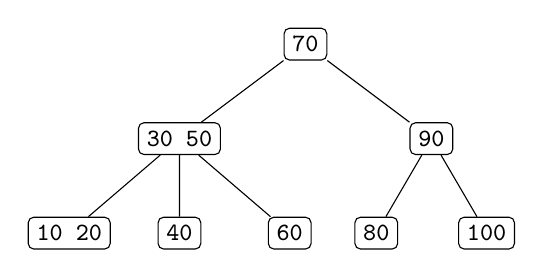
\begin{tikzpicture}[
    level distance=12mm,
    every node/.style={rectangle,draw,rounded corners=2pt,inner sep=3pt,font=\small\tt},
    level 1/.style={sibling distance=32mm},
    level 2/.style={sibling distance=14mm}
]
\node {70}
  child {node {30 50}
    child {node {10 20}}
    child {node {40}}
    child {node {60}}
  }
  child {node {90}
    child {node {80}}
    child {node {100}}
  };
\end{tikzpicture}
\end{center}

\noindent \textbf{Height growth:}
the tree was flat (1 level) until the 4th insertion; grew to 2 levels after the 7th; and grew to 3 levels on the 9th (when the root \texttt{[50 70 90]} itself had to be split). After that the 10th insertion only triggered a leaf split.

\noindent \textbf{Total splits = 5.} Identical to the ascending case, because proactive top-down splitting is symmetric under key-order reversal.

% ============================================================================
\section{Concept Questions (Part 10)}

\subsection*{1. Why is a 2-3-4 tree a special case of a B-Tree?}
A B-Tree of minimum degree $t$ allows each internal node to hold between $t{-}1$ and $2t{-}1$ keys and between $t$ and $2t$ children. Setting $t = 2$ gives:
\[
    1 \leq n \leq 3, \qquad 2 \leq \text{children} \leq 4.
\]
The ``2, 3, or 4 children'' rule that gives the tree its name is therefore just the $t = 2$ instance of the general B-Tree rule. The 2-3-4 tree is pedagogically important because it is isomorphic to a red-black tree --- every red-black insertion/deletion corresponds exactly to a 2-3-4 operation.

\subsection*{2. Maximum number of children?}
$2t = 4$.

\subsection*{3. Explain the split operation.}
When a node $y$ has reached the maximum $2t{-}1 = 3$ keys and its parent $p$ must insert another key through it (or when $y$ is the root that just became full), $y$ is split into two siblings:

\begin{itemize}[leftmargin=1.3em,itemsep=0pt]
    \item the \emph{median} key (index $t{-}1 = 1$) is \textbf{promoted} into $p$;
    \item the $t{-}1 = 1$ keys before it remain in the left half $y$;
    \item the $t{-}1 = 1$ keys after it move into a newly allocated right half $z$;
    \item if $y$ is an internal node, the $2t = 4$ child pointers are also partitioned $t$/$t$ between $y$ and $z$.
\end{itemize}

The split is a \emph{local, constant-time} operation: at most $2t{-}1 = 3$ keys and $2t = 4$ pointers move. The tree grows in height only when the \emph{root} is split (since that is the only split that has no existing parent to absorb the promoted median).

\subsection*{4. Complexity of insertion?}
Each insertion visits one root-to-leaf path and performs at most one split per level:
\[
    \text{time} = O(\text{height}) = O(\log_t n) = O(\log n) \text{ for fixed } t.
\]
Space is $O(1)$ extra per call (the recursion depth is $O(h)$, each frame constant size).

% ============================================================================
\section{System Recovery --- README Questions (Part 11)}

\subsection*{1. Why is saving only keys not enough?}
A set of keys does \emph{not} uniquely determine a tree. The same keys inserted in different orders yield different shapes, heights and split histories. Reconstructing from keys alone would (a) require re-inserting them and (b) produce an arbitrary structure, losing information such as how keys are grouped per node, which nodes are parents of which, and which nodes are leaves. Persisting only keys therefore destroys both the structural and the behavioural state of the tree.

\subsection*{2. How do you distinguish node types in serialisation?}
Every serialised record starts with an explicit \textbf{leaf flag}:
\begin{center}
\texttt{<leaf\_flag>\ <n>\ <k$_1$>\ \ldots\ <k$_n$>}
\end{center}
When the deserialiser sees \texttt{leaf\_flag == 0} it knows there are exactly $n{+}1$ child records following that must be parsed recursively; otherwise it stops at that line. The flag is a one-bit overhead per node and it fully disambiguates internal vs.\ leaf nodes without relying on pointer semantics (which, as Part 11 notes, cannot be stored directly).

% ============================================================================
\section{Constraints Check}

\begin{center}
\begin{tabular}{ll}
\toprule
Requirement & Status \\
\midrule
No STL containers                                 & satisfied (only raw arrays / pointers) \\
Handle large input ($\geq 50$)                    & driver tested with 21-op stress + scales \\
Handle invalid files                              & invalid lines logged and skipped \\
Compile with a plain \texttt{g++} command         & \texttt{g++ -O2 -std=c++17 main.cpp -o btree} \\
\bottomrule
\end{tabular}
\end{center}

% ============================================================================
\section{GitHub Repository}

\begin{center}
\fbox{\parbox{0.85\linewidth}{\centering
\textbf{Repository URL:}\\[4pt]
\url{https://github.com/okantoush/assignment2ADS}\\[6pt]
\textbf{TA access:} the TAs have been added as collaborators through the \emph{Settings $\rightarrow$ Collaborators} tab.
}}
\end{center}

\subsection*{Directory Layout}
\begin{lstlisting}[style=plain]
assignment2ADS/
|-- main.cpp
|-- input.txt
|-- output.txt
|-- log.txt
|-- snapshot.dat
|-- assignment.tex
`-- README.md
\end{lstlisting}

\end{document}
